\tikzstyle{field}=[rectangle,draw=black,line width=1pt,align=center,font=\footnotesize,minimum height=1cm]
\linespread{0.8}

\scalebox{.66}{
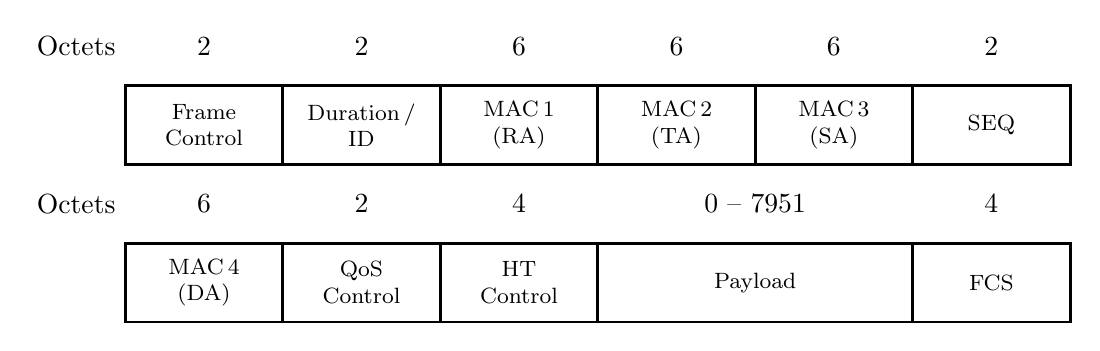
\begin{tikzpicture}[>=latex]
	%\draw (0,0) rectangle (2,1);
	\node[field,minimum width=2cm] at (0,0) {Frame\\Control};
	\node[field,minimum width=2cm] at (2,0) {Duration\,/\\ID};
	\node[field,minimum width=2cm] at (4,0) {MAC\,1\\(RA)};
	\node[field,minimum width=2cm] at (6,0) {MAC\,2\\(TA)};
	\node[field,minimum width=2cm] at (8,0) {MAC\,3\\(SA)};
	\node[field,minimum width=2cm] at (10,0) {SEQ};


	\node[field,minimum width=2cm] at (0,-2) {MAC\,4\\(DA)};
	\node[field,minimum width=2cm] at (2,-2) {QoS\\Control};
	\node[field,minimum width=2cm] at (4,-2) {HT\\Control};
	\node[field,minimum width=4cm] at (7,-2) {Payload};
	\node[field,minimum width=2cm] at (10,-2) {FCS};
	%\draw (2,0) rectangle (4,1);
	%\draw (4,0) rectangle (6,1);
	%\draw (6,0) rectangle (8,1);
	%\draw (8,0) rectangle (10,1);
	%\draw (10,0) rectangle (12,1);

	%\draw (0,-1.5) rectangle (2,-2.5);
	%\draw (2,-1.5) rectangle (4,-2.5);
	%\draw (4,-1.5) rectangle (6,-2.5);
	%\draw (6,-1.5) rectangle (10,-2.5);
	%\draw (10,-1.5) rectangle (12,-2.5);

	% Bits
	\node[left] at (-1,1) {Octets};
	\node at (0,1) {2};
	\node at (2,1) {2};
	\node at (4,1) {6};
	\node at (6,1) {6};
	\node at (8,1) {6};
	\node at (10,1) {2};
	
	\node[left] at (-1,-1) {Octets};
	\node at (0,-1) {6};
	\node at (2,-1) {2};
	\node at (4,-1) {4};
	\node at (7,-1) {0 -- 7951};
	\node at (10,-1) {4};
	%\draw (-1,1.5) node {\footnotesize Octets};
	%\draw (1,1.5) node {\footnotesize 2};
%	\draw (3,1.5) node {\footnotesize 2};
%	\draw (5,1.5) node {\footnotesize 6};
%	\draw (7,1.5) node {\footnotesize 6};
%	\draw (9,1.5) node {\footnotesize 6};
%	\draw (11,1.5) node {\footnotesize 2};

%	\draw (-1,-1) node {\footnotesize Octets};
%	\draw (1,-1) node {\footnotesize 6};
%	\draw (3,-1) node {\footnotesize 2};
%	\draw (5,-1) node {\footnotesize 4};
%	\draw (8,-1) node {\footnotesize 0 -- 7951 Byte};
%	\draw (11,-1) node {\footnotesize 4};
	

	% Fields
	%\draw (1,0.5) node {\footnotesize FC};
	%\draw (3,0.75) node {\footnotesize Dur};
	%\draw (3,0.25) node {\small ID};
	%\draw (5,0.5) node {\footnotesize MAC 1};
	%\draw (7,0.5) node {\footnotesize MAC 2};
	%\draw (9,0.5) node {\footnotesize MAC 3};
	%\draw (11,0.5) node {\footnotesize Seq};

	%\draw (1,-2) node {\footnotesize MAC 4};
	%\draw (3,-2) node {\footnotesize QoS};
	%\draw (5,-2) node {\footnotesize HT};
	%\draw (8,-2) node {\footnotesize Payload};
	%\draw (11,-2) node {\footnotesize FCS};
\end{tikzpicture}
}
